\begin{figure}[t]
\centering
  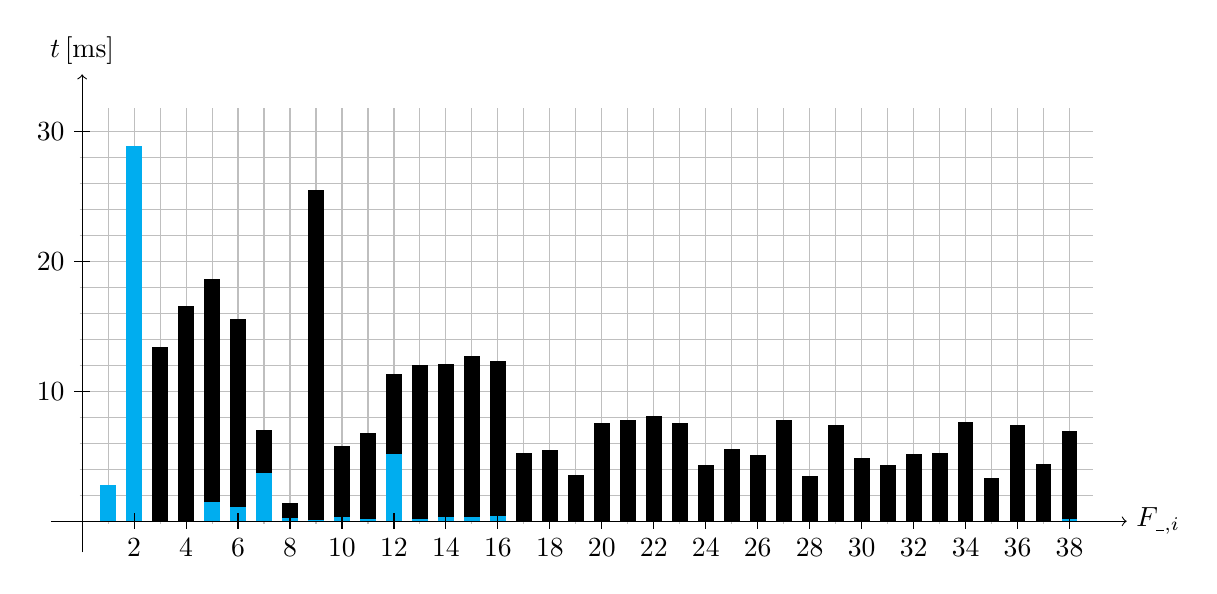
\begin{tikzpicture}[scale=0.33]
  \draw[color=lightgray] (-0.1, -0.1) grid (38.9, 15.9);
  \tikzstyle{color1}=[color=cyan]

  \def\nocachevalues{{
     2.6410,
    28.5100,
    13.3869,
    16.5449,
    18.6330,
    15.5669,
     7.0220,
     1.4099,
    25.5279,
     5.8319,
     6.8040,
    11.3669,
    11.9970,
    12.0990,
    12.6920,
    12.3380,
     5.2409,
     5.4859,
     3.5239,
     7.5699,
     7.7840,
     8.0809,
     7.5949,
     4.2960,
     5.5909,
     5.1359,
     7.8219,
     3.4979,
     7.3950,
     4.8370,
     4.3480,
     5.1550,
     5.2339,
     7.6390,
     3.3230,
     7.3960,
     4.4110,
     6.9430}}

  \def\cachevalues{{
     2.7799,
    28.8550,
     0.0019,
     0.0019,
     1.4799,
     1.0950,
     3.6849,
     0.2480,
     0.0989,
     0.3180,
     0.2019,
     5.1459,
     0.1980,
     0.3459,
     0.3060,
     0.4390,
     0.0049,
     0.0020,
     0.0029,
     0.0029,
     0.0030,
     0.0300,
     0.0309,
     0.0019,
     0.0029,
     0.0039,
     0.0029,
     0.0020,
     0.0030,
     0.0019,
     0.0040,
     0.0019,
     0.0030,
     0.0029,
     0.0029,
     0.0020,
     0.0019,
     0.2120}}

  \foreach \x in {1,...,38}
    \pgfmathparse{\nocachevalues[\x - 1] / 2}
    \edef\nocachevalue{\pgfmathresult}
    \draw[line width=0.2cm] (\x, 0) -- (\x, \nocachevalue);

  \foreach \x in {1,...,38}
    \pgfmathparse{\cachevalues[\x - 1] / 2}
    \edef\cachevalue{\pgfmathresult}
    \draw[line width=0.2cm, color1] (\x, 0) -- (\x, \cachevalue);

  \draw[->] (-1.2, 0) -- (40.2, 0) node[right] {$\ma{F}_{\_,i}$};
  \draw[->] (0, -1.2) -- (0, 17.2) node[above] {$t \left[\mathrm{ms}\right]$};

  \foreach \y in {1,...,3}
    \pgfmathtruncatemacro{\label}{10 * \y}
    \draw (0.3, 5*\y) -- (-0.3, 5*\y) node[left] {\label};

  \foreach \x in {1,...,19}
    \pgfmathtruncatemacro{\label}{2 * \x}
    \draw (2*\x, 0.3) -- (2*\x, -0.3) node[below] {\label};

\end{tikzpicture}
  \caption[]{}
\label{fig:merkmals_caching}
\end{figure}
